\documentclass[sigconf,nonacm]{acmart} % Options: sigconf, sigplan, sigchi, etc.

%% === Metadata ===
\title[Notes Drug Extraction]{Drug Dosage Extraction of Pharmacist Notes in MIMIC Using Llama for Discrepancy Flagging}
\author{Owen Wurst}
\email{owurst@utexas.edu}
\affiliation{%
  \institution{University of Texas}
  \city{Austin}
  \state{Texas}
  \country{USA}
}

\begin{document}

\begin{abstract}
There is a vast amount of error due to data discrepancies in the medical field. This bad data can lead to injury, loss of life, negative financial impacts, and regulatory issues. The purpose of this project is to evaluate the efficacy of using NLP methods, with the focus on LLM usage, to flag discrepancies between pharmacist notes and prescription data entries. Research has been done in radiology to use LLMs to find discrepancies and with drugs using classical NLP methods to extract data about drug usage from text, but research in drugs using LLMs for discrepancy analysis is missing. Using MIMIC data, I aimed to determine what type of model was best at extracting drug dosage information from pharmacy notes and also to use that model to develop a way to compare the extracted information to MIMIC prescription tables. While I was able to determine that the LLM was best at the extraction, I was unable to develop a way to complete accurate comparisons in the way required for a system that would be used to raise flags on data discrepancies. 
\\\\Code on my github \url{https://github.com/OWurst/AI_In_Healthcare_HRP}
\end{abstract}

\keywords{MIMIC3, Medical NLP, Large Language Models, Llama, Data Annotation, Machine Learning/Deep Learning}

\maketitle
\vspace*{2\baselineskip}

\section{Introduction}
The rise in the power of, the access to, and the efficiency of large language models in recent years have rapidly pushed the bounds of what is possible in the field of Natural Language Processing. In the medical field, we have vast catalogs of notes that can now be parsed by models with greater ability to summarize, comprehend, and extract information.
\\\\Medical systems are highly complex, with many errors that are considered preventable that occur due to inefficiencies within the systems. In the US alone, an estimated 400,000 patients experience preventable harm, with over 200,000 preventable deaths. Furthermore, estimates of financial loss due to preventable errors have been made of up to 45 billion USD annually. A large portion of these are medication errors, which come from bad data entry of prescriptions due to preventable things like weight entry errors, drug dosage entry errors, the wrong drug being entered because a medication sounds similar to another medication, etc. \cite{NIH}.
\\\\For this project, my aim is to flag the discrepancies between pharmacy notes and prescription tables. What this means is that I will extract drug information, such as dosage, frequency, and drug type, from the pharmacist's notes for a given patient admission and compare what the pharmacist's notes reflect with what the entered data in the prescription table is showing. I will be using python notebooks to train and utilize models to first, extract drug information from the notes, and then, with the best model, we will use the extracted information to flag instances where the notes do not match. This, if successful, would provide an immediate proof of concept for a real time system to compare medical notes to data entry not only in prescriptions, but other administrations as well. This will allow hospitals to better track inventory, identify pain points (and potentially people that need extra training) in data entry, treat patients more effectively, and identify potential fraud while building more robust datasets to build future improvements upon. Overall, intelligent systems like this will improve a hospital's ability to treat patients, spend money effectively, and comply with regulations.  

\section{Related Work}
There has been some strong related work to my goal. A large amount of research has gone into using LLMs for annotation of medical documents with one study finding that LLMs can substantially decrease the cost of human time for expert level labels with multiple models upwards of $90\%$ accuracy for NER of specific medical language\cite{goel}. This is an obvious need for us because the reason these notes are not being utilized is that its just unfeasible for people to examine all of them, so they are largely only consulted when issues already arise, rather than being used as a way to prevent issues.
\\\\Another study has specifically been done on drug information extraction from health record notes and found that NER could have some positive effect citing many of the same trends and needs to examine notes as I am, but they did not go so far as to use an LLM for this \cite{jagg}. So it appears there is a lack of utilization of LLMs for specifically the fully automated data extraction from medical notes with the focus with LLMs more being on summary, annotation, and NER and a higher use of classical NLP methods for data extraction, likely do to the speed and resource constraints that would come from using an LLM in a real-time system, at least specifically with drugs.
\\\\One study that is more in-line functionally with with my aim was a study in Sweden where researchers were able to use LLMs to flag errors in radiology reports. Researchers were able to reach at least $90\%$ for all error types in the reports as a classifier of whether the report had a discrepancy or not, and were able to classify the specific class of discrepancy $67\%$ of the time. This crushed their baseline scores and is a great example of how LLMs can be used to process large amount of complex text data in a system \cite{alfons}.

\section{Methodology}
There will be 2 parts to the experimentation because our system has 2 steps. First, we are going to compare several models of extraction, which will be just simple Regex (the baseline), Medspacy, and the LLM model Llama 3, which we expect to be the best, but don't want to use for performance reasons unless it is truly better. Then, we will compare our models and decide which one will go into our prototype real-time system. The second step will be to use the selected model in the system to extract drug data from the notes and then compare to the records in the prescription table. We will call this the Extraction Comparison Engine.

\subsection{Data}
All data used in this project will come from a large subset of MIMIC-3 data that I have loaded locally in MySQL. For legal reasons, the LLM I use will be hosted locally, as MIMIC data is regulated.
\\\\From MIMIC, we are specifically using noteevents that are of the category 'Pharmacy', because they will have the best 1:1 relationship (really one to many, as one note may have multiple drugs, but we can handle this by checking multiple records for every note) for comparison to prescription records.

\subsection{Extraction Model Comparison}
For this first step of analysis, we are going to use the top 10 most common drugs in the prescription table and extract information from noteevents that contain them. This leaves us 26 noteevents to examine. We will use 3 types of models.

\subsubsection{Regex}
As a baseline we will start with a non-AI based extraction. Using a sliding window, we will look for certain terms nearby our target drug names and see what we find. Within 20 characters of our target drug we search for number and unit patterns to try and extract data from the text.

\subsubsection{Medspacy}
An upgrade to the plain regex method, we next will use Named Entity Recognition with surrounding regex. Medspacy is a medical model that can be used for NER to specifically locate drugs in a set of text. By locating the drug that is the focus of a text based on context and finding the units that surround it, we can improve upon just a simple text match for a drug, which can happen many times in a text, and instead find the instance of the drug that the note is about, separately, one time for each drug. We still use a regex window to find the surrounding numeric values and units.

\subsubsection{Llama}
The last model is our LLM. This model is a locally hosted Llama-3 8B parameter model that you can download through gpt4all. The model is relatively lightweight but still quite powerful. For this method of extraction, we get rid of all regex and instead provide a prompt asking for structured results in a specific format. The prompt example code is provided in figure 1. We still provide the list of drugs to look for, but we have escaped the need for a window and instead trust the model to get some understanding of the text.

\begin{figure}[t]
    \centering
    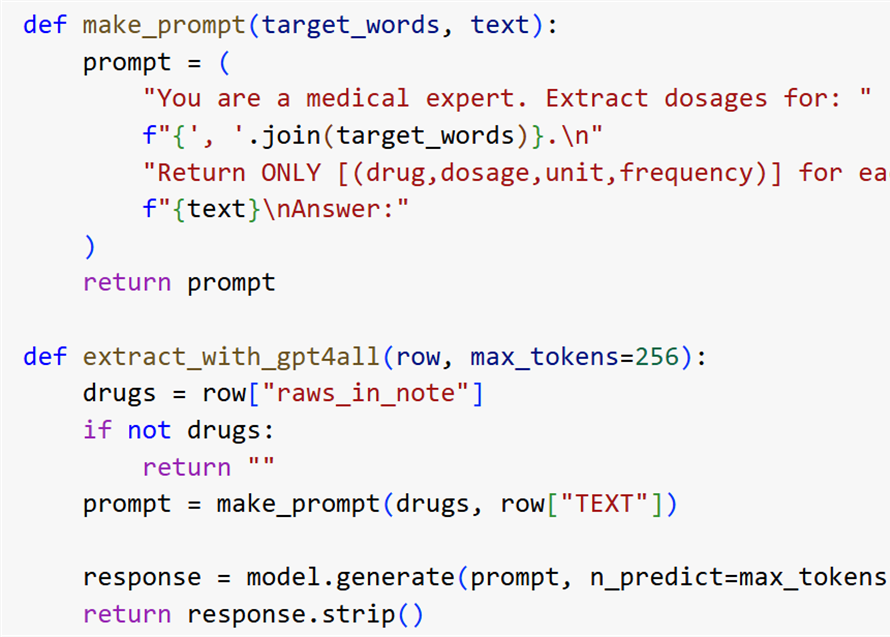
\includegraphics[width=.8\linewidth]{prompt_code.png}
    \caption{Prompt Example}
    \label{fig:prompt}
\end{figure}

\begin{figure}[t]
  \centering
  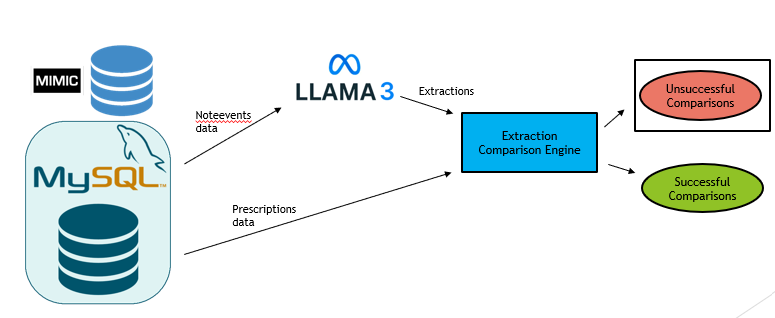
\includegraphics[width=\linewidth]{experiment_diagram.png}
  \caption{System pipeline for extraction and discrepancy flagging}
  \Description{This diagram shows the different components and how data flows sequentially from left to right. On the left we have our mimic data stored in MySQL. Moving right, we pull notes and prescriptions. Notes are put into Llama3 which is prompted to perform the extraction, and these extractions are compared to the prescriptions table, we flag all misclassifications}
  \label{fig:pipeline}
\end{figure}

\subsection{Extraction Comparison With Llama}
Figure 2 shows the sequential left-to-right data flow. On the left, MIMIC data are stored in MySQL. Moving right, we pull notes and prescriptions. Notes are sent to Llama 3, which is prompted to perform dosage extraction; these extractions are compared to the \texttt{PRESCRIPTIONS} table, and any mismatches are flagged as discrepancies. Looking closely at the Llama outputs, we can see some discrepancy in the formatting the LLM has given us our extractions in, for now this will have to be handled by the extraction comparison engine code.
\\\\Extraction comparison was by far the most difficult process in this code. Many notes that do not have discrepancies with the prescription records get flagged for using different names for the same drug, different units for dosages, and different spacings, language, etc, even in the prescriptions table which is meant to be raw data. A large portion of the extraction comparison engine code is focused on parsing different dosages, drug names, and units across various prescription table columns to deal with inconsistencies in how data is input. We could flag all of these, which in a real time system MAY prompt a hospital to improve data entry processes, but I think overwhelming people with a new system is more likely to cause lack of adoption and instead I want to focus on finding true positive failures and minimizing false positives. Thus, the code is meant to flag note/record pairs where there is definitely a discrepancy.

\section{Results}
Once again, we have two result sections because our results for the methodology in 3.2 (results found in 4.1) will influence the methodology in 3.3 which I would say gives us the true overarching results for the entire experiment in 4.2. 

\subsection{Extraction Results}

\subsubsection{Regex}
The plain regex method has provided a lot of results, with most result sets including the correct extraction; however, there are duplicate extractions and conflicting extractions with no way to identify which is the best extraction. The regex will always output every instance where a drug, say lorazepam shows up near any dosages, so we get extractions that say 2mg, 1mg, 1mg/hr, all for the same text.

\subsubsection{Medspacy}
Medspacy is producing better results and less results. We see much less duplicates and conflicting extractions for a specific text, with target drugs being located less times based on their NER tag; however, we are getting notes where we failed to correctly tage any of the target drugs. So while we have more accurate results, we have less results.

\subsubsection{Llama}
The Llama model took much longer to run than the others, but it has done a much better job. Llama outputs 1 decision per target drug in the text and has successfully gotten a result for every text, which we know all had at least one instance of a target drug. One interesting thing it did was that it also output results for drugs found in the text that were not target drugs.

\subsection{Extraction Comparison Results}
In figure 3 we can see the overall results. Out of 554 pharmacy notes, we had 505 get flagged for data inaccuracy. We can see that examples of the matches are actually true matches, but our real target population, the mismatches, seems to show only examples where we didn't have an expected drug from the prescriptions table. Also, if we look at figure 4, we can see that there is not a single instance where the drug matched but some other value did it.

\begin{figure}[t]
  \centering
  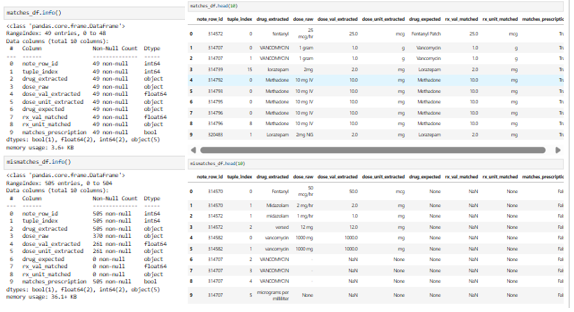
\includegraphics[width=\linewidth]{results.png}
  \caption{Results: Stats and examples of Mismatches (Discrepancies) and Matches}
  \Description{This diagram shows the different components and how data flows sequentially from left to right. On the left we have our mimic data stored in MySQL. Moving right, we pull notes and prescriptions. Notes are put into Llama3 which is prompted to perform the extraction, and these extractions are compared to the prescriptions table, we flag all misclassifications}
  \label{fig:results}
\end{figure}

\begin{figure}[t]
  \centering
  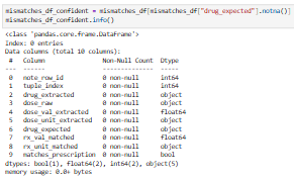
\includegraphics[width=\linewidth]{mismatches.png}
  \caption{Results: Mismatches Where there was a Match for Drug Name}
  \Description{Diagram shows pandas info for a df made by taking all mismatches where expected drug name is not null, there are 0}
  \label{fig:pipeline}
\end{figure}

\section{Discussion}
\subsection{Extraction Discussion}
Unsurprisingly, the LLM has performed the best. Regex and NER with medspacy had superior speed and were easier to make work on any hardware, but the increase in success is, in my opinion, very worth it. The reliance on regex in both of the first two models makes it likely to pick up extraneous data, especially in more complex and unusually structured texts, and therefore these models cannot be robust unless you want to tune them on every type of document you expect to see for hyperparameters like window size. Even then, you are not going to beat the understanding capability of the LLM. I will continue with the LLM as the tool for the focus of the project, which is the comparison of these extractions to prescription data.

\subsection{Extraction Comparison Discussion}
While some of the missing drugs are likely true examples of one class of discrepancy we are looking for, where a pharmacist notes a drug but it is never entered in the prescriptions table, it is highly unlikely that such a strong majority can be this way, and that it could be the only type of error. It is much more likely that I am missing critical MIMIC data to this (from my own process of importing MIMIC data, not the MIMIC discrepancies that we are looking for) and that I need to better flesh out the comparison cases or come up with a new way to develop these rules, as it is not a simple task to take an extraction and see if it matches in the prescription table.

\section{Conclusion and Future Work}
Overall, I have to concede that this iteration of this methodology has been a failure. While there has been some success in showing that there is strong opportunity to use LLMs for data extraction of medical notes specifically regarding drugs. We have failed in our attempt to build a proof of concept for a real-time system that would be able to flag these discrepancies, as we almost entirely failed to flag these discrepancies as a whole; however, I think there are some key things to fix that I would like to pursue before scrapping this idea entirely.
\\\\First, we need to fix data issues that are not specific to MIMIC. Due to hardware constraints, I have only downloaded a subset of all of the MIMIC data. Although this set of data is still large, it is likely we are missing prescription records that are needed to compare to noteevents.
\\\\Second, I need to more clearly define success metrics to evaluate the system as a whole. So far, I have only been able to test by examining results, which is rather ineffective. To evaluate the efficacy system as a whole, I will need to define accuracy metrics for both the model used for the extraction and for the extraction comparison engine.
\\\\Last, I need to more rigorously test both the extraction process and the comparison engine separately before combining. I need to tune prompts to be more precise and get better structured results from the LLM. For the comparison engine, I need a large unit test suite to ensure I am handling all the edge cases with missing data properly, as this is the place I most attribute my failure too, there is simply so much going on with this missing data that the level of rules required for how to handle/convert different units, drug names, columns that drug names are in, etc. This needs to be fixed, as it is the portion of the pipeline that will be truly unique to each individual use case and likely every hospital outside of MIMIC.
\\\\In conclusion, I have failed, but I have seen some promising evidence that the idea could still work and I do see a relatively straightforward, albeit time consuming, path to fixing the most glaring issues. For this reason, I think that there is enough to build upon for future work.

\begin{acks}
I would like to thank Dr. Ying Ding and all the TAs, especially Monte Jarvis. I also thank gpt4all \url{https://www.nomic.ai/gpt4all} for having free access to high performance lightweight LLMs that can be hosted locally.
\end{acks}

\bibliographystyle{ACM-Reference-Format}
\bibliography{references}
\nocite{*}

\end{document}